\section{Provenance Audit and Identification Targets}
\label{sec:formulation}
Consider an acquisition episode with task $x$, trajectory $\tau$, and terminal outcome $z\in\{0,1\}$. Let $P\in\{S,F\}$ denote whether the source trajectory succeeded or failed. In a provenance-conditioned memory system, $P$ can affect at least two downstream objects: the writer mode $W(P)$ used to construct memory and, when exposed to the agent, a provenance label or metadata field $L(P)$. The written memory is
\begin{equation}
M = G(\tau,W(P)),
\end{equation}
and future behavior follows
\begin{equation}
Y = H(x',M,L,S),
\end{equation}
where $x'$ is the future query and $S$ is the remaining agent state. ReasoningBank instantiates the writer channel directly: successful trajectories are analyzed under a success-reflection objective, while failed trajectories are processed under a failure-reflection objective \citep{ouyang2026reasoningbank}. A system may also attach an explicit provenance field to the resulting memory.

\begin{figure}[t]
\centering
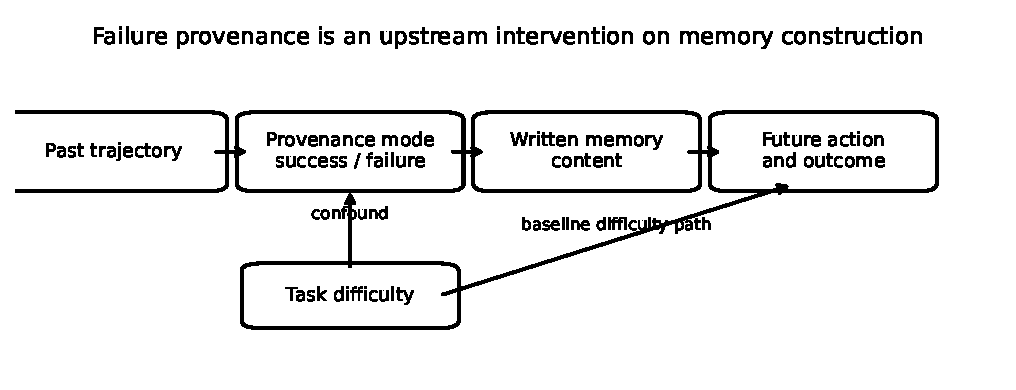
\includegraphics[width=\linewidth]{figures/fig1_provenance_causal.pdf}
\caption{Coarse causal structure of provenance-conditioned memory. Acquisition difficulty can affect both source outcome and later task performance. Writer mode mediates the path from source provenance to written memory; an optional visible provenance-metadata channel is omitted for readability. Matching future queries and semantic guidance reduces the task-difficulty confound but does not make generated memories identical.}
\label{fig:causal}
\end{figure}

\subsection{A provenance effect is not a single estimand}
The observational quantity
\begin{equation}
A_P = \mathbb{E}[Y\mid P=S]-\mathbb{E}[Y\mid P=F]
\end{equation}
is useful as an audit signal, but it is not causal: acquisition difficulty $D$ can influence both $P$ and future outcomes. More importantly, a notation such as $do(P)$ is underspecified once provenance controls memory construction. One must state which downstream channel is intervened on.

The \emph{writer-mode contrast} changes the reflection objective while fixing the future query and released observation state:
\begin{equation}
\Delta_W(x') =
\mathbb{E}[Y\mid do(W=W_F),x',E,\mathcal{G}=1]-
\mathbb{E}[Y\mid do(W=W_S),x',E,\mathcal{G}=1],
\label{eq:writer}
\end{equation}
where $E$ denotes the frozen future evidence/state and $\mathcal{G}$ is a preregistered information-equivalence gate on the two generated memories. This is the object approximated by our R4 and R6 bridges. Even when $\mathcal{G}=1$, the intervention can change wording, emphasis, decomposition, or other decision-relevant properties of $M$; therefore $\Delta_W$ is a writer-mode-bundle estimand, not automatically a provenance-metadata-only effect.

A stricter \emph{exact-information provenance-exposure contrast} holds actionable memory content, retrieval membership, and retrieval order fixed, and changes only whether truthful source-outcome provenance is visible to the executor. For a retrieved memory set $m$ with truthful provenance vector $p$, define
\begin{equation}
\Delta_L(m,x') =
\mathbb{E}[Y\mid M=m,do(L=p),x',E]-
\mathbb{E}[Y\mid M=m,do(L=\varnothing),x',E].
\label{eq:metadata}
\end{equation}
This is an incremental-information estimand: it asks whether exposing provenance adds value beyond the same actionable content, rather than assuming that SUCCESS or FAILURE has a fixed sign. Historical R5 targets the same rung but support-stops before model execution. The fresh R53--R57 experiment executes this contrast prospectively on 32 independent MemRL/OSInteraction clusters.

\subsection{Provenance-audit identification ladder}
Table~\ref{tab:ladder} turns these distinctions into a reusable audit protocol. The key reporting rule is that request count is not automatically the inference unit: R4 contains 48 completed requests but only four independent task units; R6 contains 276 requests but 23 independent task units.

\begin{table}[t]
\centering
\caption{Provenance-audit identification ladder.}
\label{tab:ladder}
\scriptsize
\begingroup
\setlength{\tabcolsep}{2pt}
\begin{tabular}{p{0.06\linewidth}p{0.34\linewidth}p{0.25\linewidth}p{0.25\linewidth}}
\toprule
Rung & Intervention / hold fixed & Current evidence and independent unit & Strongest allowed claim \\
\midrule
L0 & Observe provenance strata; no intervention & Financial audit; source/retrieval cases & Association / audit signal only \\
L1 & Switch writer mode; fix future query/state; require $\mathcal{G}=1$ & R4: 4 task pairs; R6: 23 task pairs & Writer-mode-bundle contrast, not provenance-only \\
L2 & Fix retrieval/content/order; hide vs expose truthful provenance & R56: 32 fresh paired clusters, 64/64 arms & Incremental terminal value of visible provenance on this substrate \\
L3 & Repeat L1/L2 in original model/runtime/source artifacts & Financial AgentDojo replication debt & Transport evidence only \\
\bottomrule
\end{tabular}
\endgroup
\end{table}

\subsection{Decision rule and completed L2 resolution}
The historical L1 gates use a frozen $|\Delta|\geq0.15$ relevance floor and task-level randomization tests; R4's four tasks imply minimum exact one-sided $p=1/16$, while R6 misses both magnitude and significance. The fresh L2 experiment separately freezes 32 paired clusters, an absolute practical-relevance floor of 0.15, a two-sided exact paired sign test, and a 100,000-resample paired-cluster bootstrap interval before the first primary treatment. It completes all 64 arms. The observed B-minus-A terminal effect is $0.03125$, with one B-only success, no A-only success, exact $p=1.0$, and preregistered bootstrap interval $[0,0.09375]$; the practical floor is not met. We therefore report qualified low incremental terminal value rather than a directional provenance benefit or a proof of exact zero.

\subsection{Identification statements}
Let $Y_W(w)=H(x',G(\tau,w),L_0,S)$ denote the potential outcome under writer mode $w$ with metadata fixed at $L_0$, and let $Y_L(\ell;m)=H(x',m,\ell,S)$ denote the potential outcome under provenance surface $\ell\in\{\varnothing,p\}$ with actionable memory set $m$ fixed exactly.

\paragraph{Proposition 1 (rung validity).} (i) L0 does not identify either $\Delta_W$ or $\Delta_L$ without an ignorability assumption for source provenance, because a latent acquisition difficulty can jointly affect $P$ and $Y$. (ii) Within a preregistered L1 admitted set, if writer mode is the only manipulated channel, future state $E$ is fixed, and consistency/no-interference hold, the paired task-level contrast identifies the finite-set writer-mode effect $\mathbb{E}[Y_W(W_F)-Y_W(W_S)]$ for that admitted set. (iii) L1 does not identify $\Delta_L$ when $G(\tau,W_F)\neq G(\tau,W_S)$. (iv) Under L2, if retrieved actionable content is byte-identical, retrieval membership/order are fixed, and executor-visible provenance is the only manipulated channel, the paired task-level contrast identifies $\mathbb{E}[Y_L(p;m)-Y_L(\varnothing;m)]$ for the evaluated substrate. L3 changes the target domain, not the intervention channel, so transport assumptions are additional to (ii)--(iv).

The non-upgrade in (iii) is constructive: two response functions can agree on every L1-observed point $(M_S,L_0)$ and $(M_F,L_0)$ yet differ arbitrarily on the unobserved metadata counterfactuals $(m,L_S)$ and $(m,L_F)$. Thus no amount of L1 replication alone determines an L2 effect. For our L1 gate, malformed memories, answer leakage, insufficient embedding similarity, verifier-detected actionable asymmetry, or a unique task-solving fact are rejected before outcomes; this narrows the writer-mode bundle but does not supply the missing equality assumption. Consequently a strong L0 signal cannot be promoted to L1/L2, a non-decisive L1 result cannot rescue L2, and an L2 support failure is not counterevidence. The rung and independent unit are therefore part of the claim, not bookkeeping.
